% Template created by Adrienne Traxler (adrienne.traxler@wright.edu)
% Last modified: 3/22/17: Add clarifying note about why the template has too much space around its section headers.
% 
% Changelog
% 3/14/17: add 2-column figure example, tweak text to align with Word sample file, add hyperref for links/cross-references
% 6/21/16: 	Fix old PACS option and superscript affiliations.
% 5/5/16: 	Update sample table to use the REVTEX ruledtabular environment for auto-sizing;
%   		switch to using pra option until the prstper style is fixed (who knows when).
% 5/10/16: Swap suggested department/institution ordering in \affiliation lines.
% 5/12/16: Remove PACS line (deprecated).
% 6/21/16:	Switch to noshowpacs and add superscriptaddress in documentclass options.
% 
% This is my best effort to follow the Physical Review style guide plus specific changes 
% required for PERC (mostly, omitting article titles in references). This version compiles 
% with pdfLaTeX alone; using a proper .bib file changes the bibliography part at the end 
% and would require running BibTex as well.
%
% Finally, there's extra padding around section headers if you compile the bare template. 
% I believe that's because LaTeX stretches its white space to keep the floats (tables and 
% figures) near their input locations. The excess spacing goes away when a normal amount 
% of body text is filled in.

% Big list of reference documentation is here: http://journals.aps.org/revtex, 
%  see especially the APS Author Guide PDF link.

% Notes on the revtex4-1 documentclass options used: 
%  reprint does the double-column, publication ready appearance
%  prstper style formats reference numbers incorrectly, fast fix is to use pra instead.
%  Add longbibliography option to show article titles (and see note in bibliography)

%\documentclass[english,aps,prstper,reprint,showpacs]{revtex4-1}   % This version should work (prstper option), but actually formats reference numbers incorrectly.
\documentclass[english,aps,pra,reprint,noshowpacs,superscriptaddress]{revtex4-1}   
% Using pra instead of prstper gives correct square-bracket (not superscript) reference formatting
\usepackage[T1]{fontenc}	% should generally be included for better accented-word behavior
\usepackage[latin9]{inputenc}	% should generally be included for better accent behavior
\usepackage{geometry}		% for controlling page margins
\geometry{verbose,tmargin=1in,bmargin=1in,lmargin=0.75in,rmargin=0.75in}	% define margins
\usepackage{graphicx}
\usepackage[above,below]{placeins}	% allows use of \FloatBar­rier command to force section barriers
\usepackage{times}
% Next three lines are optional, use the hyperref package to make URLs and reference links live.
\usepackage{hyperref}  
\hypersetup{colorlinks=true,urlcolor=blue,citecolor=blue,linkcolor=blue}   
\urlstyle{same}
\pagestyle{empty}			% page numbers added later, when compiling the whole proceedings
\begin{document}

\title{Paradigms in Physics 2.0}
\author{David Roundy}
\author{Liz Gire}
\author{Ethan Minot}
\author{Emily van Zee}
\affiliation{Department of Physics, Oregon State University, Corvallis, Oregon, 97331}
\author{Tevian Dray}
\affiliation{Department of Mathematics, Oregon State University, Corvallis, Oregon, 97331}
\author{Corinne A. Manogue}
\affiliation{Department of Physics, Oregon State University, Corvallis, Oregon, 97331}

%\keywords{}

\begin{abstract}
In 2016, the Department of Physics at Oregon State University began a
process to revise our Paradigms in Physics curriculum for physics
majors.  This poster will describe both the process by which our
department achieved consensus on this curricular change, and the
resulting curriculum.  The Paradigms 2.0 committee begain with a
survey of students and faculty, followed by individual interviews with
the faculty teaching each existing course.  As we developed a plan to
address student- and faculty-identified challenges in the curriculum,
we met with each faculty member individually to explain and refine our
proposal, which was unanimously approved by the faculty.  Major
changes include elimination or major changes to several courses (math
methods, computational physics, modern physics, electronics, and
classical mechanics), including the introduction of two sophomore-year
courses designed specifically to help prepare students to for their
upper-division courses.
\end{abstract}

\maketitle

\section{Introduction}
The Paradigms in Physics program is a rethinking of the upper-division
physics curriculum that began around the time when our current
students were born~\cite{manogue2001paradigms}.  The basic ideas
behind the original Paradigms reform were (1) attention to the
sequencing of concepts, (2) acheiving faculty buy-in, which requires
faculty to understand the sequencing, and (3) implementation of active
engagement through the upper-division curriculum.  In 2016, we began a
rethinking of the Paradigms, with focus on the same principles guiding
the original effort, but with the input of new faculty, and applying
lessons learned over the past two decades.  In this paper, we will
explain the reasoning behind this Paradigms 2.0 effort, the process by
which we achieved developed and reached consensus on an improved
curriculum, and will give both a summary and a few highlights of the
new program.

\subsection{Background}
The Paradigms in Physics project began in 1996, when three faculty
members at Oregon State applied to the NSF for funding to redesign the
upper-division curriculum.  The motivation for the original Paradigms
project was in fact similar to the motivation for Paradigms 2.0: a
desire to soften the ``brick wall'' encountered by students upon
reaching the junior year, within the constraint that transfer students
must be able to graduate with two years of upper-division
courses~\cite{manogue2001paradigms}.  The process of redesigning the
curriculum was dominated by the creation index cards listing subject
content, and sorting these cards into courses.  This process involved
the entire faculty, and culminated in a unanimous agreement to adopt
the resulting curriculum.

The resulting curriculum was primarily composed of junior-year
``Paradigms'' courses, followed by senior-year ``Capstone'' courses.
The Paradigms were intensive 2-credit, 3-week courses which meet every
day, for a total of seven hours per week.  Paradigms incorporate
laboratory experiences and active engagement into the class, and
typically have two problem sets per week.  Capstones were more
traditional 3-credit courses which meet three hours per week for an
entire quarter.  The Paradigms courses had integrated math content,
followed by a Math Methods course.

A coupe of decades have passed since the original Paradigms effort.
During this time we have made a number of changes: e.g. a new
\emph{first} Paradigm was introduced to soften the beginning of the
junior year, the order of Paradigms was shuffled more than once, Math
Methods was moved from the beginning of the senior year to the end of
the junior year, and a computational laboratory course was introduced
to accompany the Paradigms.  We maintained the tradition of meeting
every three weeks to discuss issues relating to upper-division
teaching.  New faculty arrived and learned to teach the new courses,
and introduced their own approach to the courses.

\subsection{Motivation for Paradigms 2.0}
There were a number of factors that motivated us to embark on the
Paradigms~2.0 process.  In the last two decades, we have observed
challenges students face in the Paradigms.  While in many cases we
addressed these by changing and reordering the courses, we felt a look
at the entire curriculum was in order.  In addition, our faculty
buy-in and aware was diminishing by attrition: while our younger
faculty are enthusiastic about the Paradigms, many lack perspective on
where students are in a given course, and what content is essential
for students to grasp prior to a following course.

\paragraph{Transfer students}
Our curriculum is strongly affected by our desire to accomodate
transfer students from community colleges.  This leads us to focus on
a physics major in which all upper-division courses are taken in two
years.  However, our current curriculum is very hard on students in
the fall of their junior year, and especially so for transfer
students.  So we aimed to structure the courses such that non-transfer
students could be better prepared for their junior year, while
transfer students could postpone a few courses so that their junior
Fall would be no more difficult than that of any other student.

\paragraph{Coupled curricular changes}
A backlog of curricular changes have accumulated that could not be
separated from an examination of the curriculum as a whole.  Most
notable were discussions of the requirements for computational
physics, the amount of required electronics credits, and the role of
our modern physics course.  These persistent issues were not easily
addressed without addressing the physics major curriculum as a whole,
and any discussion of one tended to devolve into a discussion of
everything, without progress being made.

\paragraph{New faculty}
At this stage, (XX) of our faculty was not present during the orignal
Paradigms effort.  Many of the newer faculty have only a superficial
undertanding of our course structure.  This poses a challenge when
these professors teach courses that are closely intertwined with one
another.

\section{Paradigms 2.0 process}
We began the Paradigms 2.0 process in the Winter of 2016, having in
the previous year obtained faculty agreement, and support from our
Department head.  The process was spearheaded by a committee of four
(the authors DR, LG, EM, and CAM, with EvZ present at meetings
documenting our process).  During the Winter quarter, we informed the
community of our process through a colloquium, and collected student
and faculty perspectives on the existing curriculum.  We then
interviewed faculty who recently taught each of our existing courses
to document topics that were currently covered.  This resulted in a
total of XXX index cards in YYY stacks, corresponding to courses, with
cards color coded by broad topic.

The committee met for ??? weeks to discuss existing challenges and
sort the cards into new stacks corresponding to new and reordered
courses.  When we discussed major changes to a course, we often
invited interested faculty to join us to provide their own perspective
on possible challenges and improvements.  Once we had a draft
proposal, we began inviting each faculty member in to see the cards
and discuss the proposed sequence of courses.  In addition, we had a
meeting with all the current students to explain the proposed changes
and request feedback.

When we had obtained feedback from the entire faculty, we scheduled
\emph{two} faculty meetings (DURATION?).  In the first meeting, we
presented our proposal in detail.  This was needed for several
reasons.  Those faculty we met with first may not have seen the final
proposal.  Some faculty during their individual meetings chose to
focus on a small subset of the curriculum, often relating to courses
they had themselves taught.  In one meeting we presented the proposal
and fielded questions.  In a second faculty meeting, we again
presented our proposal, and opened the floor for discussion.  After
considerable discussion, we unanimously voted to adopt the proposed
changes.

%\newcommand\mathcourse[2]{\emph{#1 (#2)}}
\newcommand\mathcourse[2]{\emph{#1}}
\newcommand\noted[2]{\textbf{#1} (#2)}
\newcommand\paradigm[1]{{\sc #1} (3)}
\newcommand\capstone[1]{#1 (3)}
\newcommand\onecredit[1]{#1 (1)}
\newcommand\threecredit[1]{#1 (3)}
\newcommand\fourcredit[1]{#1 (4)}

\begin{figure*}
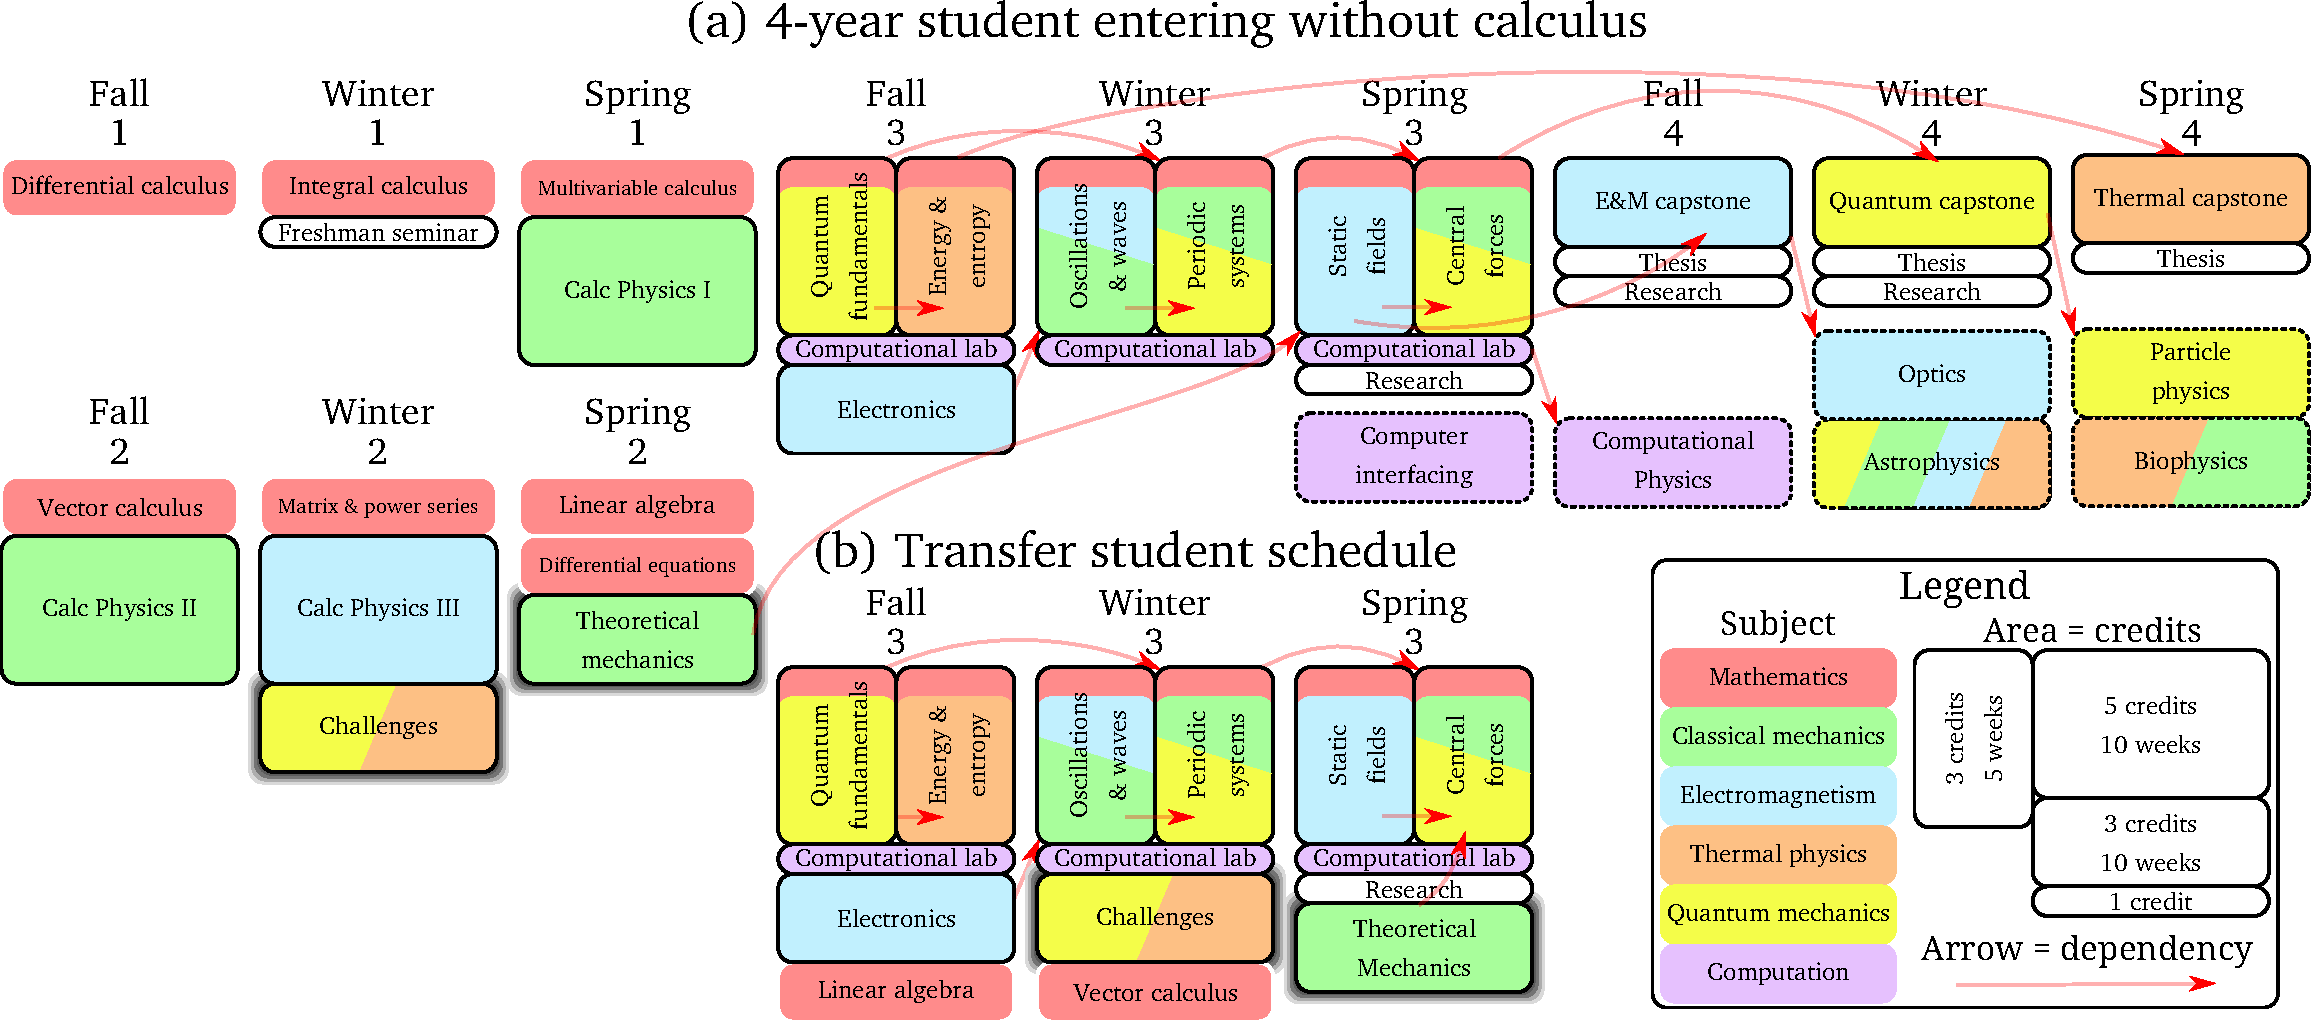
\includegraphics[width=\textwidth]{schedule}
\caption{Hypothetical student schedules for (a) a student entering
  without calculus and (b) a transfer student.  The Dependencies
  between courses are noted with arrows.  The area of each course is
  proportional to the credit value of the course, with the exception
  of math courses, which are shown in small boxes even though they are
  4-credit courses.  The two newly introduced courses are indicated
  with shadows.\label{fig:schedule}}
\end{figure*}

\section{Changes made}
As a result of this process, we have implemented a number of changes
to our physics major curriculum.  The resulting curriculum is outlined
in Fig.~\ref{fig:schedule}.  The changes consisted of introducing two
new sophomore-level courses (which may be taken in the junior year) to
better prepare our majors for the Paradigms.  We eliminated Modern
Physics and the Classical Mechanics capstone in favor of the two new
sophomore-level courses.  We eliminated the Math Methods course in
favor of ``math bits'' integrated into the Paradigms themselves.
Finally, we restructured our nine 3-week Paradigms courses into six
5-week Paradigms.  We changed our computational physics requirement,
and reduced the number of electronics courses.

\subsection{5-week Paradigms}
To begin with the most distinctive feature of our curriculum, we
wanted to maintain the existing intensive 7-hour-per-week schedule in
the junior year, which we have found effective.  However, we chose to
change from three 3-week Paradigms per quarter to two 5-week Paradigms
per quarter.    This change has several advantages.  It gives students
a bit more time with each professor prior to their final exam.  This
gives a bit more flexibility, for instance, in case of illness.
Finally, by reducing the number of Paradigms, we allow the curriculum
to be taught with fewer faculty, albeit at a work load per professor.

We put considerable thought into the content and ordering of the new
Paradigms.  In most cases, we think of each 5-week Paradigm as either
one formerly 4-week Paradigm (the one that consumed the extra week
each quarter) or two 3-week Paradigms compressed.  The major
scheduling change is to place Static Fields (electrostatics and
magnetostatics) in the spring quarter.  This intended to give students
a bit more time to take Vector Calculus.  It also puts all use of
curvilinear coordinates in the spring quarter, which should ease the
learning of Central Forces.  The final major change was the
elimination of special relativity from the Paradigms, which is has now
moved into the new sophomore-level Theoretical Mechanics course.

\subsection{Math bits}
We chose to eliminate the Math Methods course in favor of formal
``math bits'' in the Paradigms.  Our previous Math Methods Capstone
posed a challenge regarding placement in the curriculum: it needed to
be sufficiently late in order for students to be adequately prepared
for advanced mathematical content, but in order to be functional in
the curriculum it should teach content that is required by other
physics courses, and thus should be earlier in the curriculum.  In
response to these issues, and in recognition that the majority of our
majors are not bound for graduate school, and have no need for
advanced math methods, we chose to integrate the needed math content
into the Paradigms, and allow advanced students to take our
graduate-level Math Methods course.  In order to ensure that our
students to receive the math instruction they require, and based on
our previous experience with math-intensive weeks (the ``odd'' weeks)
in the Paradigms, we chose to integrate one week of ``math bits'' into
each Paradigm.  The math bits for the entire year are treated as a
distinct teaching assignment, so students will be accustomed to the
treatment of math as a distinct subject supporting the physics
content.  This provides some relief from teaching for the Paradigms
professors, and at the same time ensures that they do not succumb to
the temptation to short-change the math content to the detriment of
the students.

\subsection{Electronics}
We chose to reduce the Electronics requirement from two 3-credit
courses to one 3-credit course.  For many physics majors, this is more
than sufficient, and gives students a greater number of electives.  In
addition, we removed the lecture section of this course---which had
developed an unusually high student work load for a 3-credit
course---in favor of in-lab instruction.

A final change to Electronics is that we now will \emph{require}
Electronics during the junior year (specifically as a prerequisite for
Oscillations and Waves).  This is made possible by the reduction in
Fall workload for incoming transfer students, who had previously
usually taken Electronics as a senior.  This change has enabled us to
articulate distinct and sequenced learning outcomes from these two
courses, particularly in the realm of complex exponentials and Fourier
transforms.  It is also beneficial in providing students with
trouble-shooting skills prior to the in-class labs taught in
Oscillations and Waves.

\subsection{Computational lab}
Over the last six years, we have been developing a 1-credit
computational laboratory course that accompanies the Paradigms.  We
chose to require this course, while removing a requirement for a
lower-division 3-credit course in computational physics.  This
lower-division course was challenging to teach, since it always had a
mix of lower- and upper-division students, with very different skill
levels and needs.  Transfer students now take computation alongside
the non-transfer students, in a laboratory setting using pair
programming to help new programmers to learn.

\subsection{Sophomore courses}
We introduced two new sophomore-level courses: \emph{Challenges in
  Contemporary Physics}, and \emph{Theoretical Mechanics}.  Both of
these courses ramp up student mathematical abilities prior to their
junior year.  The Challenges course will focus on estimation,
dimensional reasoning, and interpretation of integrals, while
Theoretical Mechanics will teach power series approximations, and
expose students to increased levels of mathematical sophistication.

These courses \emph{will} have the challenge (which was removed from
the computational course!) of teaching both juniors and sophomores
together.  They will be taught in the winter and spring quarters, so
as to reduce the burden on transfer students in the Fall.  They were
explicitly constructed to \emph{not} teach any content required for
Fall or Winter Paradigms so that they can be taken concurrently with
the Paradigms.

\subsubsection{Challenges in Contemporary Physics}

In ``The Physics of Contemporary Challenges'' we prepare students to
apply physics concepts and physical reasoning skills to sustainable
energy issues, climate change mechanisms, space exploration and
puzzles in fundamental physics. These ``real-world'' topics are chosen
for either the societal need (energy and climate), and/or the human
need to explore (space and fundamental physics). By prioritizing
inclusion of the most engaging challenges, we aim to attract and
retain as many potential physics majors as possible.

While contemporary challenges determine the narrative flow of the
course, physics concepts and physical reasoning skills are the main
substance. Students are introduced to thermodynamics, statistical
mechanics, electromagnetic radiation, quantum mechanics, and modern
experimental physics---in each case motivated by one or more
``contemporary challenges''. Together with new physics concepts,
students are given new reasoning tools, such as the equipartition
theorem, the quantum-classical correspondence principle, order of
magnitude calculations, simplifying assumptions, and numerical
integration. Mathematically rigorous derivations are only briefly
discussed in class, with additional details offered in online video
format. In summary, we emphasis the physics concepts and reasoning
skills that allow professional physicists to quickly/quantitatively
make an initial assessment of a complex problem.

The students engage with the material by solving daily quiz questions
in class, solving weekly homework problems, performing a modern
physics experiment, and writing a term paper. The daily quiz questions
help clarify the goal of each lecture. The weekly homework questions
are directly related to contemporary challenges are require a variety
of estimation techniques. The modern physics experiment, performed
with a low cost kit (LEDs, diffraction grating, rulers, volt meter
etc.) emphasizes a quantitative approach to observation and explores
issues of experimental uncertainty. Lastly, the term paper allows
students to dive deeper into a particular contemporary challenge. The
term paper tests student's ability to make their own initial
assessment of a complex problem, and communicate their ideas with
diagrams, graphs and estimations.

%% Climate change and renewable energy are major contemporary
%% challenges. Students are inspired to engage with these challenges, and
%% physics will play a critical role in addressing these challenges.
%% Former Energy Secretary Steve Chu recently noted that ``physics majors
%% seem to be increasing,'' and pointed to millennials' interests in the
%% risks of climate change, clean energy, and
%% sustainability~\cite{kramer2016gathering}.  However, most majors get
%% little or no interaction with such challenges in their physics
%% classes.

%% We have introduced a course that fits seamlessly into the physics
%% major sequence, that focuses on the contemporary challenges of
%% sustainable energy and climate change. The course will be a bridge
%% between introductory physics and upper-division classes for both
%% physics majors and students from related disciplines such as chemistry
%% and engineering. The challenges theme will motivate the introduction
%% of thermal physics and quantum mechanics as well as the development of
%% physical reasoning skills. We anticipate that an emphasis on the role
%% of physics in overcoming societal challenges will help us recruit and
%% retain a greater number of physics majors, especially women and
%% under-represented minorities.

%% At Oregon State, as at many other universities, a course in Modern
%% Physics traditionally bridges the lower and upper divisions and serves
%% as an introduction to quantum mechanics. Such courses typically follow
%% a historical narrative, celebrating the achievements of men like
%% Planck, Einstein, Rutherford, Bohr, Bragg, Millikan, de Broglie,
%% Pauli, Schroedinger, and Dirac. Indeed, it is a wonderful and exciting
%% story - and inspiring for those who imagine themselves as
%% reincarnations of these men. However, we suggest that this historical
%% narrative does not attract a wide cross-section of participants to
%% physics. Instead, we have introduced a forward-looking narrative that
%% emphasizes the relevance of physics today unconstrained by the details
%% of the great transition from 1905 to 1945.

%% Each physics topic is linked to contemporary challenges. An
%% understanding of electromagnetic waves is required to understand how
%% light interacts with vibrational modes of CO$_2$. The equipartition
%% theorem explains the heat energy stored in the ocean. Quantum
%% mechanics explains the blackbody spectrum, semiconductor electronic
%% structure, and solar photovoltaics. The Carnot cycle convinces us that
%% a 95\%-efficient gas furnace cannot compete with an efficient heat
%% pump.

%% The new perspectives associated with this course, along with an
%% emphasis on expanding students' reasoning skills, will strengthen the
%% connection between lower- and upper-division physics classes. Students
%% will learn the importance of approximate calculations (Fermi
%% estimates) that establish reasonable bounds on the exact
%% answer. Students will learn that equations help us interpret the
%% physical world, i.e. equations are used for much more than mindless
%% algebraic manipulations.  Students will learn how integration and
%% differentiation can be applied to real data - not just the perfect
%% functions that are taught in math class. Students will learn how
%% graphing of relationships is key tool for physicists. The utility of
%% these skills will be firmly established by application to contemporary
%% challenges.

\subsubsection{Techniques of Theoretical Mechanics}

While the Challenges courses takes a more experimental/applied physics
focus, the Methods of Theoretical Mechanics course has a more
theoretical physics flavor. The theme of this course is the discussion
of strategies for making sense of physics problems and symbolic
problem solving. This sense-making includes coordinating and
interpreting symbolic expressions with conceptual understandings,
geometric relationships, and physical intuitions.

This Theoretical Mechanics course is aimed at students who are taking
or have completed the last course in the introductory sequence. The
physics content of the course is advanced Newtonian mechanics,
introduction to Lagrangian and Hamiltonian techniques, and special
relativity. These topics at this stage for the students are convenient
for explicit discussion of sense-making strategies in physics because
(a) students are have recently studied problems that serve as limiting
cases for more complex problems, (b) students at this level are
transitioning from solving problems primarily involving numbers to
problems with only symbolic parameters, and (c) we can discuss
sense-making as strategies for approaching a problem, evaluating
answers, and refining intuitions about relativistic and other
unfamiliar situations. For example, we teach students how to use
spacetime diagrams to develop a story about a relativistic situation
and how to use hyperbola trig on these diagrams to perform Lorentz
transformations that can be checked against the results of algebraic
Lorentz transformations.  The sense-making goals of the course are on
equal footing with the physics goals, and sense-making is integrated
explicitly in all aspects of the course: exams, homework and during
in-class activities. Our aim is that students will develop
sense-making skills that will improve their learning in advanced
courses and will impress their upper-division course instructors,
research advisors, and future employers.

%% To physicists, mathematics is a language for telling stories about
%% conceptual physical relationships.  Our understandings of conceptual
%% connections guide us when we manipulate
%% equations~\cite{gire2008resources, bing2007cognitive,
%%   wittmann2015mathematical}[75].  For example, when solving ordinary
%% differential equations by separating variables, we choose limits of
%% integration so that the lower (and upper) limits for all variables
%% describe the same physical state.  We monitor algebraic manipulations
%% using conceptual understandings of physics quantities. For example, we
%% make sure that each term in a sum has the same physical dimensions
%% (e.g. you can't add a frequency to a frequency squared). We make sure
%% that expressions on both sides of an equals sign have the same
%% dimensions~\cite{lenz2016dimensional}. We consider limiting cases to
%% make sure that a derived expression reasonably describes the system in
%% extreme states~\cite{singh2002physical}. Our geometric understandings
%% guide the formulation of equations~\cite{gire2014arrows}. Sometimes,
%% we do not have adequate mathematics to describe complex physical
%% systems. We use conceptual understandings to make choices about
%% reasonable idealizations in order to create useful mathematical
%% models~\cite{bing2007cognitive}.

%% Being fluent in this physics language involves both (1) translating a
%% conceptual story into a mathematical representation and (2) discerning
%% a conceptual story from a mathematical
%% representation~\cite{tuminaro2007elements}. At the introductory level,
%% students often see concepts and mathematics as being separate. These
%% students do not expect equations to help their conceptual
%% understanding~\cite{adams2006new, redish1998expectations} and have
%% trouble formulating equations from a conceptual analysis. Students who
%% do not have mathematical fluency for physics struggle in advanced
%% physics courses~\cite{manogue2009cognitive}.

%% We propose a course that explicitly focuses on physics majors'
%% mathematical fluency and sense-making skills. Introductory courses
%% begin to develop these aspects, but the primary goals of those courses
%% tend to be for students to apply simple concepts (Newton's Laws,
%% energy conservation, etc.) to relatively straightforward and very
%% idealized problems.

%% This course is taken either just after or concurrently with the last
%% quarter of the introductory physics sequence. It leverages students'
%% understandings of simple mechanical systems from introductory physics
%% to develop their mathematical fluency in the context of less
%% idealized, more sophisticated systems. Each physics topic
%% (velocity-dependent forces, Lagrangian mechanics, Hamiltonian
%% mechanics, special relativity) will focus on specific math methods
%% (e.g. differential equations, calculus of variations, generalized
%% coordinates, Legendre transformations, linear transformations,
%% hyperbola geometry) and will explicitly feature strategies to make
%% physical sense of mathematics (symbolic problem solving, reading
%% equations like sentences, making idealization, coordinating
%% representations, limiting case analysis, dimensional checking).

\section{Summary}
We have developed a significant incremental change to the Paradigms
curriculum.  This change focused on the first two big ideas underlying
the Paradigms: (1) close attention to content ordering, and (2)
developing a consensus and understanding of the curriculum among our
faculty members.  Our commitment to using active engagement in our
upper-division curriculum remains unchanged.  While the specific
content ordering we developed is interesting, the \emph{process} by
which we reached it, and developed a faculty consensus is at the
essence of what makes distinctive the Paradigms in Physics program.
The process of developing faculty understanding of the Paradigms is
ongoing, as we are having professors new to the Paradigms shadow
experienced faculty as they teach in the Paradigms, prior to teaching
the courses themselves..

Future work will involve documenting the learning trajectories that we
have developed in our curriculum.  Furthermore, we are engaging in a
project to study our students' development of sense-making skills in
particular through the two new courses that are intended specifically
to ramp up those skills (instincts?).

We look forward to another two decades of the Paradigms!

% Formatting tweak if needed--FloatBarrier forces floats to show here, before next section
%\FloatBarrier	


\acknowledgments{This work was supported by the National Science
  Foundation under Grant No. 1323800 Supplement.}

% For a longer bibliography, delete the thebibliography block above, then comment in 
% these two lines to use a .bib file with BibTeX.
\bibliographystyle{apsrev}  	% supercedes the longbibliography option, so leave commented out if you want to display article titles
\bibliography{paper}  	% don't include the .bib suffix

%% \begin{table*}[htbp]
%% \caption{Hypothetical student schedule for a student entering without
%%   calculus.  Students with AP Calculus can take the junior-year
%%   courses one year earlier, and students who start calculus-based
%%   physics in the Fall of their second year are not
%%   delayed.\label{schedule}}
%% \begin{ruledtabular}
%% \begin{tabular}{rlll}
%%   \textbf{Year} & \textbf{Fall} & \textbf{Winter} & \textbf{Spring} \\
%%   \hline
%%   1 & \mathcourse{Differential calculus}{251} &
%%   \mathcourse{Integral calculus}{252} &
%%   \mathcourse{Multivariable calculus}{254} \\
%%     & & \onecredit{Freshman Seminar} & \fourcredit{Calc Physics I} \\
%% \hline  2 & \mathcourse{Vector calculus}{255}
%%   & \mathcourse{Differential equations}{256}
%%   & \mathcourse{Linear algebra}{341} \\
%%   & \fourcredit{Calc Physics II} & \fourcredit{Calc Physics III} &\mathcourse{Series \&
%%     sequences}{253} \\
%%   && \noted{Challenges}{3} & \noted{Theoretical Mechanics}{3}
%%   \\
%% \hline 3 & \paradigm{Quantum fundamentals} & \paradigm{Osciallations \& waves} & \paradigm{Static fields}
%% \\
%%   & \paradigm{Energy \& entropy} & \paradigm{Periodic systems} & \paradigm{Central forces}
%% \\
%%   & \onecredit{Computational lab I} & \onecredit{Computational lab II} & \onecredit{Computational lab III}
%% \\
%%   & \threecredit{Electronics} & \threecredit{Computer interfacing} & \onecredit{Research}
%% \\
%% \hline 4 & \capstone{Electromagnetism capstone} & \capstone{Quantum capstone} & \capstone{Thermal capstone}
%% \\
%% & \onecredit{Thesis} & \onecredit{Thesis} & \onecredit{Thesis}
%% \\
%% & \onecredit{Research} & \onecredit{Research}
%% \end{tabular}
%% \end{ruledtabular}
%% \end{table*}

%% \begin{table*}[htbp]
%% \caption{Hypothetical transfer student schedule.  Most transfer
%%   students will have a heavier schedule in their transfer year due
%%   to need to catch up on required math courses.\label{schedule}}
%% \begin{ruledtabular}
%% \begin{tabular}{rlll}
%%   \textbf{Year} & \textbf{Fall} & \textbf{Winter} & \textbf{Spring} \\
%%   \hline
%% 3 & \paradigm{Quantum fundamentals} & \paradigm{Osciallations \& waves} & \paradigm{Static fields}
%% \\
%%   & \paradigm{Energy \& entropy} & \paradigm{Periodic systems} & \paradigm{Central forces}
%% \\
%%   & \onecredit{Computational lab I} & \onecredit{Computational lab II} & \onecredit{Computational lab III}
%% \\
%%   & \threecredit{Electronics} & \threecredit{Computer interfacing} & \onecredit{Research}
%% \\
%% & \mathcourse{Linear algebra}{341} & \noted{Challenges}{3} & \noted{Theoretical Mechanics}{3}
%% \\
%% &&\mathcourse{Vector calculus}{255}
%% \\
%% \hline 4 & \capstone{Electromagnetism capstone} & \capstone{Quantum capstone} & \capstone{Thermal capstone}
%% \\
%% & \onecredit{Thesis} & \onecredit{Thesis} & \onecredit{Thesis}
%% \\
%% & \onecredit{Research} & \onecredit{Research}
%% \end{tabular}
%% \end{ruledtabular}
%% \end{table*}

\end{document}
